% !TEX program = xelatex
\documentclass[aspectratio=169, 11pt]{beamer}

% ── Theme & Colors ──────────────────────────────────────────────────────────
\usetheme{Madrid}
\usecolortheme{default}

% ── Packages ────────────────────────────────────────────────────────────────
\usepackage{amsmath, amssymb}
\usepackage{booktabs}
\usepackage{tikz}
\usetikzlibrary{arrows.meta, positioning, calc}
\usepackage{graphicx}
\usepackage{listings}
\usepackage{fontspec}
\usepackage{tabularx}
\usepackage{xeCJK}

% ── Chinese Font Configuration ─────────────────────────────────────────────
\setCJKmainfont{Noto Sans CJK SC}
\setCJKsansfont{Noto Sans CJK SC}
\setCJKmonofont{Noto Sans Mono CJK SC}

% ── Title ───────────────────────────────────────────────────────────────────
\title[LLM12: Inference \& KV-Cache]{LLM12: LLM Inference --- Decoding Strategies \& KV-Cache}
\subtitle{AUP Learning Cloud --- AMD Research}
\author{CS290W}
\date{\today}

% ════════════════════════════════════════════════════════════════════════════
\begin{document}

% ── Title Slide ─────────────────────────────────────────────────────────────
\begin{frame}
	\titlepage
\end{frame}



% ════════════════════════════════════════════════════════════════════════════
\section{Two-Stage Inference Pipeline}
% ════════════════════════════════════════════════════════════════════════════

\begin{frame}{Two-Stage Inference Pipeline}


	\begin{block}{Prompt Phase (Prefill)}
		\begin{itemize}
			\item Process entire prompt in parallel
			\item Compute-bound: high arithmetic intensity
			\item Latency: Time to First Token (TTFT)
		\end{itemize}
	\end{block}

	\begin{block}{Token Generation Phase (Decode)}
		\begin{itemize}
			\item Generate one token at a time (sequential)
			\item Memory-bound: low arithmetic intensity
			\item Throughput: tokens per second
		\end{itemize}
	\end{block}

\end{frame}

% ────────────────────────────────────────────────────────────────────────────
\begin{frame}{Autoregressive Generation}


	\textbf{Autoregressive generation}: given a prompt, generate one token at a time.

	\begin{center}
		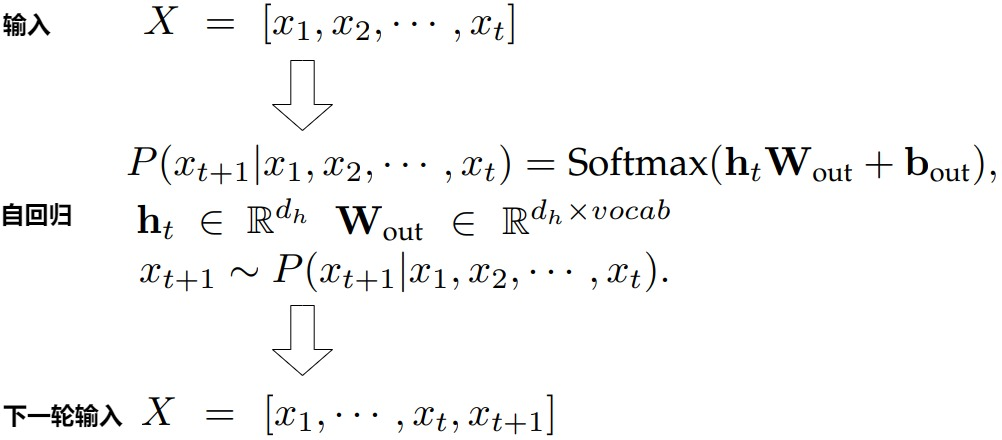
\includegraphics[width=0.6\textwidth]{img/kv-autoregressive.jpg}
	\end{center}



\end{frame}

% ────────────────────────────────────────────────────────────────────────────
\begin{frame}{Why Decode is Memory-Bound}

	\textbf{Key insight}: Decode loads the \textbf{entire model weights} for just \textbf{one token}.

	\begin{columns}[T]
		\begin{column}{0.48\textwidth}
			\begin{block}{Model Weight Access}
				\begin{tabular}{@{}lc@{}}
					\toprule
					\textbf{Stage}       & \textbf{Weights/token} \\
					\midrule
					Prefill ($s$ tokens) & $\frac{16h^2 L}{s}$    \\
					Decode (1 token)     & $16h^2 L$              \\
					\bottomrule
				\end{tabular}

				\vspace{0.3cm}
				Qwen3-0.6B: weights $\approx$ 1.2\,GB \\
				At 30\,tok/s: $\sim$36\,GB/s bandwidth!
			\end{block}
		\end{column}
		\begin{column}{0.48\textwidth}
			\begin{block}{KV-Cache Access}
				\begin{tabular}{@{}lc@{}}
					\toprule
					\textbf{Stage} & \textbf{KV read/step}  \\
					\midrule
					Prefill        & Write only             \\
					Decode         & Read all $s$ positions \\
					\bottomrule
				\end{tabular}

				\vspace{0.3cm}
				At $s$=8192: $\sim$0.9\,GB per decode step
			\end{block}
		\end{column}
	\end{columns}

\end{frame}

% ────────────────────────────────────────────────────────────────────────────
\begin{frame}{Arithmetic Intensity}

	\textbf{Arithmetic intensity} = FLOPs / bytes loaded $\rightarrow$ determines compute vs.\ memory bottleneck.

	\begin{center}
		\begin{tabular}{@{}lccccc@{}}
			\toprule
			\textbf{Stage} & \textbf{Seq Len} & \textbf{FLOPs} & \textbf{Bytes}   & \textbf{Ratio}& \textbf{Intensity}                                     \\
			\midrule
			Prefill        & 128              & 92B            & 0.97GB         & 95 & \quad\textcolor{green!60!black}{\textbf{compute}}   \\
			Prefill        & 8192             & 13.5T          & 2.8GB          & 4779 & \quad\textcolor{green!60!black}{\textbf{compute}} \\
			\midrule
			Decode         & 128              & 719M           & 0.97GB         & 0.74 & \quad\textcolor{red}{\textbf{memory}}             \\
			Decode         & 8192             & 1.6B           & 2.8GB          & 0.58 & \quad\textcolor{red}{\textbf{memory}}             \\
			\bottomrule
		\end{tabular}
	\end{center}

	\begin{alertblock}{Implication}
		Prefill processes many tokens in parallel $\rightarrow$ high intensity $\rightarrow$ GPU is busy.\\
		Decode processes 1 token $\rightarrow$ low intensity $\rightarrow$ GPU is idle, waiting for data.
	\end{alertblock}

\end{frame}

% ════════════════════════════════════════════════════════════════════════════
\section{Decoding Strategies}
% ════════════════════════════════════════════════════════════════════════════

\begin{frame}{From Logits to Tokens}

	The model outputs logits $z \in \mathbb{R}^{|V|}$. How do we pick the next token?

	\begin{block}{Temperature Scaling}
		$$\tilde{p}_i = \frac{\exp(z_i / T)}{\sum_j \exp(z_j / T)}$$
		\begin{itemize}
			\item $T < 1$: sharper $\rightarrow$ more deterministic
			\item $T > 1$: flatter $\rightarrow$ more random
			\item $T \to 0^+$: approaches greedy
		\end{itemize}
	\end{block}

	\begin{columns}[T]
		\begin{column}{0.48\textwidth}
			\begin{block}{Top-K Sampling}
				Keep only $k$ highest-probability tokens, re-normalize.
			\end{block}
		\end{column}
		\begin{column}{0.48\textwidth}
			\begin{block}{Top-P (Nucleus) Sampling}
				Keep smallest set with cumulative prob $\geq p$.
			\end{block}
		\end{column}
	\end{columns}

	\textbf{Typical pipeline}: Temperature $\rightarrow$ Top-K $\rightarrow$ Top-P $\rightarrow$ Sample

\end{frame}

% ────────────────────────────────────────────────────────────────────────────
\begin{frame}{Decoding Strategy Comparison}

	\textbf{Demo}: 10-token vocabulary, logits = [2.0, 1.5, 1.0, 0.5, 0.0, -0.5, -1.0, -1.5, -2.0, -3.0]

	\begin{center}
		\small
		\begin{tabular}{@{}ll@{}}
			\toprule
			\textbf{Strategy}   & \textbf{Unique tokens sampled (20 trials)} \\
			\midrule
			T=0.3 (sharp)       & [0, 1, 2]                                  \\
			T=1.0 (default)     & [0, 1, 2, 3, 4, 6, 7]                      \\
			T=2.0 (flat)        & [0, 1, 2, 3, 4, 5, 6, 7, 9]                \\
			Top-K=3             & [0, 1, 2]                                  \\
			Top-P=0.8           & [0, 1, 2, 3]                               \\
			T=0.7 + K=5 + P=0.9 & [0, 1, 2]                                  \\
			\bottomrule
		\end{tabular}
	\end{center}

	\begin{itemize}
		\item Greedy always picks token 0 (highest logit)
		\item Lower temperature $\rightarrow$ less diversity
		\item Top-K/P restrict the candidate set
	\end{itemize}

\end{frame}

% ────────────────────────────────────────────────────────────────────────────
\begin{frame}{Temperature Effect Visualization}

	\begin{center}
		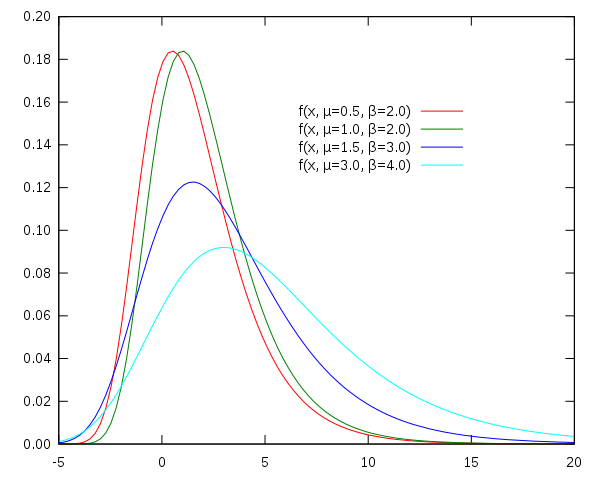
\includegraphics[width=0.4\textwidth]{img/temperature-softmax-dist.png}
	\end{center}

	\begin{block}{Temperature Control}
		\begin{itemize}
			\item \textbf{Low $T$}: High confidence, low diversity (good for factual QA)
			\item \textbf{Medium $T$}: Balanced creativity and coherence
			\item \textbf{High $T$}: High diversity, lower quality (good for brainstorming)
		\end{itemize}
	\end{block}

\end{frame}

% ────────────────────────────────────────────────────────────────────────────
\begin{frame}{Top-K vs Top-P Comparison}

	\begin{columns}[T]
		\begin{column}{0.48\textwidth}
			\begin{block}{Top-K (e.g., K=3)}
				\begin{itemize}
					\item Sort tokens by probability
					\item Keep only top $K$ tokens
					\item Re-normalize probabilities
					\item Sample from restricted set
				\end{itemize}
				\begin{alertblock}{Issue}
					Fixed $K$ may be too restrictive or too loose depending on distribution shape.
				\end{alertblock}
			\end{block}
		\end{column}
		\begin{column}{0.48\textwidth}
			\begin{block}{Top-P / Nucleus (e.g., P=0.9)}
				\begin{itemize}
					\item Sort tokens by probability
					\item Accumulate until sum $\geq P$
					\item Dynamic candidate set size
					\item More adaptive than Top-K
				\end{itemize}
				\begin{alertblock}{Advantage}
					Automatically adjusts to distribution: few tokens for confident predictions, more for uncertain.
				\end{alertblock}
			\end{block}
		\end{column}
	\end{columns}

\end{frame}

% ────────────────────────────────────────────────────────────────────────────
\begin{frame}{Repetition Penalty Example}

	Models can produce repetitive text. Three penalty mechanisms:

	\begin{block}{Repetition Penalty (HuggingFace)}
		For each previously seen token: divide logit if positive, multiply if negative.
	\end{block}

	\begin{block}{Presence Penalty (OpenAI)}
		Subtract a constant from any previously seen token's logit.
	\end{block}

	\begin{block}{Frequency Penalty (OpenAI)}
		Subtract value proportional to how many times the token appeared.
	\end{block}

	\begin{center}
		\small
		\begin{tabular}{@{}lrr@{}}
			\toprule
			\textbf{Token 0 (appears 3$\times$)} & \textbf{Original} & \textbf{After penalty} \\
			\midrule
			Rep penalty=1.5                      & 3.0               & 2.00                   \\
			Freq=0.5 + Pres=0.3                  & 3.0               & 1.20                   \\
			\bottomrule
		\end{tabular}
	\end{center}

\end{frame}

% ════════════════════════════════════════════════════════════════════════════
\section{KV-Cache}
% ════════════════════════════════════════════════════════════════════════════



% ────────────────────────────────────────────────────────────────────────────
\begin{frame}{What is KV-Cache?}

	\textbf{Problem}: Without cache, each decode step recomputes K/V for \textbf{all} past tokens.

	\begin{center}
		\begin{tikzpicture}[
			node distance=0.6cm,
			box/.style={draw, rounded corners, minimum width=1.5cm, minimum height=0.8cm, align=center, font=\scriptsize},
			arr/.style={-{Stealth[length=2mm]}, thick}
			]
			\node[box, fill=blue!15] (q) {$Q_{\text{new}}$};
			\node[box, fill=red!15, right=0.5cm of q] (k) {$K_{\text{all}}$};
			\node[box, fill=green!15, right=0.5cm of k] (v) {$V_{\text{all}}$};

			\node[below=0.3cm of q, font=\scriptsize, gray] {new token};
			\node[below=0.3cm of k, font=\scriptsize, gray] {recomputed!};
			\node[below=0.3cm of v, font=\scriptsize, gray] {recomputed!};

			\node[box, fill=red!25, right=2cm of k, minimum width=3cm] (cache) {KV-Cache\\(stored from past)};
			\draw[arr, dashed, accentblue] (k.east) -- (cache.west);
		\end{tikzpicture}
	\end{center}

	\begin{block}{KV-Cache Optimization}
		Cache past K/V tensors. During decode, only project the \textbf{new} token's K/V.\\
		Append to cache: $K = [K_{\text{cache}}; K_{\text{new}}]$, $V = [V_{\text{cache}}; V_{\text{new}}]$
	\end{block}

\end{frame}

% ────────────────────────────────────────────────────────────────────────────
\begin{frame}{KV-Cache Memory Allocation}

	\begin{columns}[T]
		\begin{column}{0.48\textwidth}
			\begin{block}{Contiguous Allocation}
				\begin{itemize}
					\item Pre-allocate fixed-size array
					\item Simple indexing: $\text{cache}[layer][position]$
					\item \textbf{Problem}: Wasted space if sequences vary in length
				\end{itemize}
			\end{block}
		\end{column}
		\begin{column}{0.48\textwidth}
			\begin{block}{Paged Attention (vLLM)}
				\begin{itemize}
					\item Divide KV-Cache into fixed-size blocks (e.g., 16 tokens)
					\item Allocate blocks on-demand
					\item Non-contiguous memory $\rightarrow$ no internal fragmentation
				\end{itemize}
			\end{block}
		\end{column}
	\end{columns}

	\begin{block}{Benefit}
		PagedAttention eliminates memory waste from padding $\rightarrow$ higher batch sizes $\rightarrow$ better GPU utilization.
	\end{block}

\end{frame}

% ────────────────────────────────────────────────────────────────────────────
\begin{frame}{KV-Cache Quantization}

	\textbf{Observation}: KV-Cache values don't need full FP16 precision.

	\begin{center}
		\small
		\begin{tabular}{@{}lccc@{}}
			\toprule
			\textbf{Format} & \textbf{Bytes/value} & \textbf{Memory} & \textbf{Quality} \\
			\midrule
			FP16 (baseline)  & 2  & 100\%  & Full precision    \\
			FP8              & 1  & 50\%   & Minimal loss      \\
			INT8             & 1  & 50\%   & Small degradation \\
			INT4             & 0.5 & 25\%  & Noticeable loss   \\
			\bottomrule
		\end{tabular}
	\end{center}

	\begin{alertblock}{FP8 KV-Cache}
		Modern GPUs (H100, MI300X) support FP8 natively.\\
		50\% memory reduction with negligible quality impact.
	\end{alertblock}

\end{frame}

% ────────────────────────────────────────────────────────────────────────────
\begin{frame}{KV-Cache Implementation}

	\begin{center}
		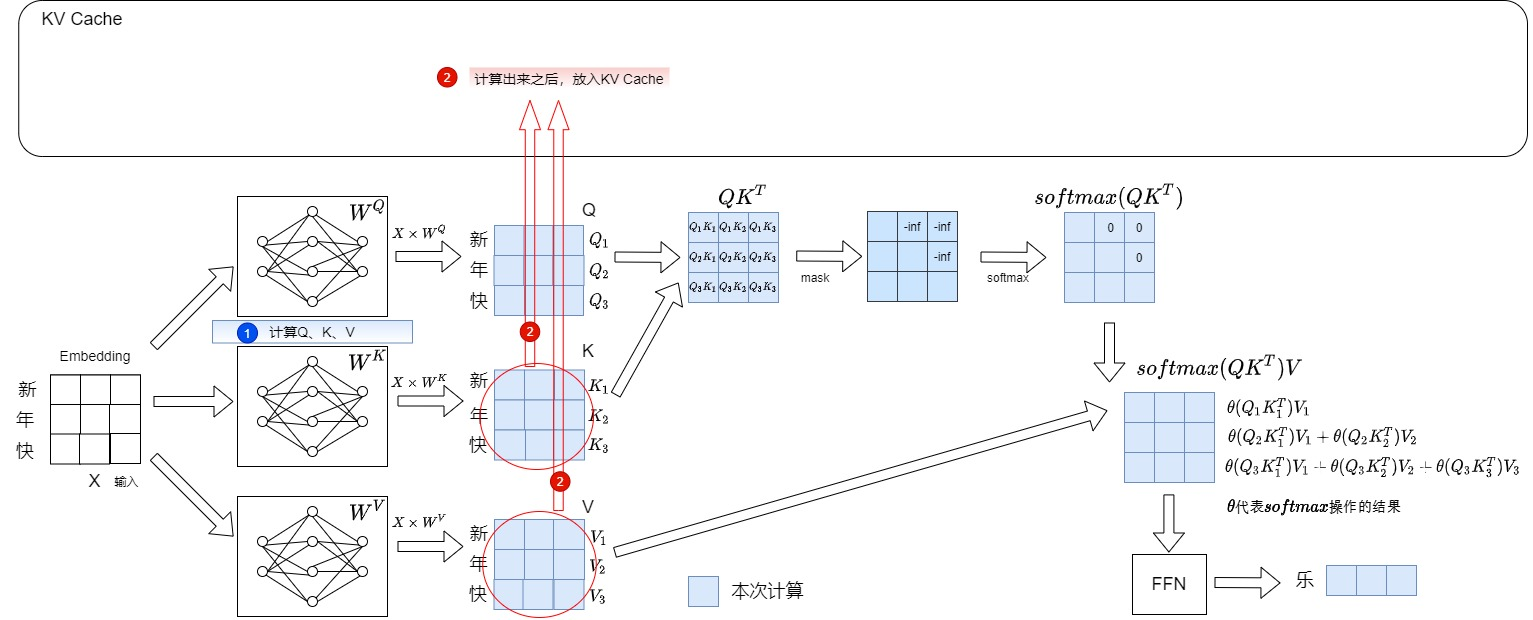
\includegraphics[width=0.6\textwidth]{img/kv-cache-flow.jpg}
	\end{center}

	\begin{block}{Key Steps}
		\begin{enumerate}
			\item Compute Q, K, V from input embeddings
			\item Store K, V in KV Cache for future reuse
			\item Compute attention using cached K, V
			\item Append new K, V to cache after each decode step
		\end{enumerate}
	\end{block}

\end{frame}

% ────────────────────────────────────────────────────────────────────────────
\begin{frame}{KV-Cache Step-by-Step Data Flow}

	\textbf{Step 1}: Input "新" $\rightarrow$ Compute Q, K, V $\rightarrow$ Output "年"

	\begin{center}
		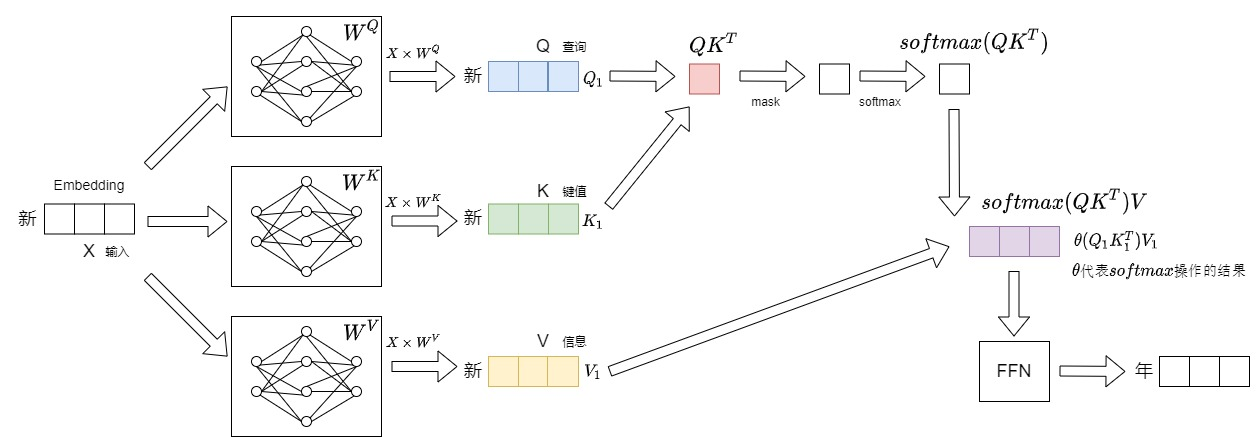
\includegraphics[width=\textwidth]{img/kv-step1.jpg}
	\end{center}

	\begin{block}{Key Observation}
		First token: no cache available, compute everything from scratch.
	\end{block}

\end{frame}

% ────────────────────────────────────────────────────────────────────────────
\begin{frame}{KV-Cache Step 2: Reuse Cached K/V}

	\textbf{Step 2}: Input "新年" $\rightarrow$ Reuse cached K/V for "新" $\rightarrow$ Output "快"

	\begin{center}
		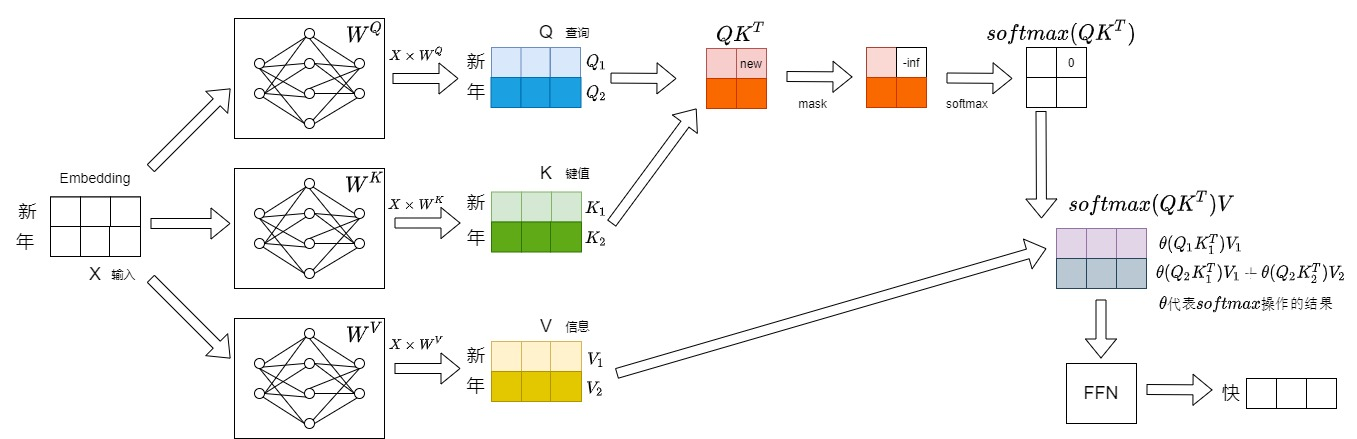
\includegraphics[width=0.8\textwidth]{img/kv-step2.jpg}
	\end{center}

	\begin{block}{Cache Reuse}
		\begin{itemize}
			\item \textcolor{red}{Red circles}: Repeated computation without cache
			\item With cache: only compute K/V for new token "年"
			\item Reuse cached K/V for "新"
		\end{itemize}
	\end{block}

\end{frame}

% ────────────────────────────────────────────────────────────────────────────
\begin{frame}{KV-Cache Step 3: Cumulative Benefit}

	\textbf{Step 3}: Input "新年快" $\rightarrow$ Reuse cached K/V for "新年" $\rightarrow$ Output "乐"

	\begin{center}
		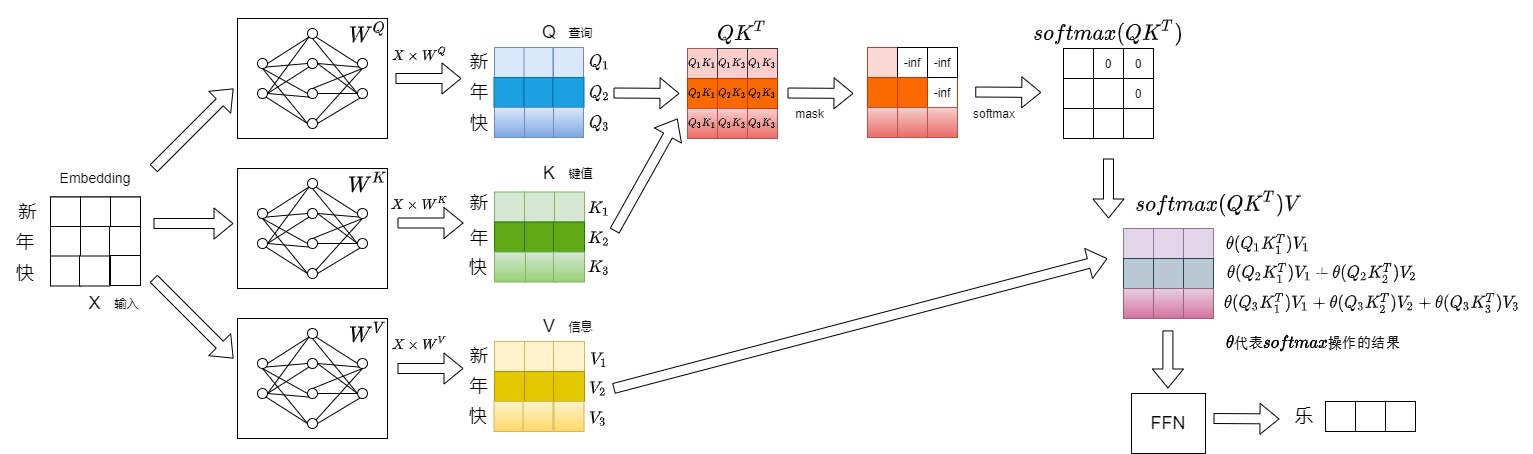
\includegraphics[width=0.8\textwidth]{img/kv-step3.jpg}
	\end{center}

	\begin{alertblock}{Growing Benefit}
		\begin{itemize}
			\item Cache contains K/V for all previous tokens
			\item Only compute K/V for the newest token
			\item Complexity reduced from $O(s^2)$ to $O(s)$
		\end{itemize}
	\end{alertblock}

\end{frame}

% ════════════════════════════════════════════════════════════════════════════
\section{KV-Cache Memory Analysis}
% ════════════════════════════════════════════════════════════════════════════

\begin{frame}{KV-Cache Memory Formula}

	For a model with GQA ($H_{\text{kv}}$ KV heads):

	$$\text{KV memory} = 2 \times b \times L \times H_{\text{kv}} \times s \times d_{\text{head}} \times \text{dtype\_bytes}$$

	\begin{center}
		\small
		\begin{tabular}{@{}lrr@{}}
			\toprule
			\textbf{Seq Length} & \textbf{KV Memory (FP16)} & \textbf{Per Layer} \\
			\midrule
			512                 & 67 MB                     & 4 MB               \\
			2,048               & 268 MB                    & 17 MB              \\
			8,192               & 1.0 GB                    & 67 MB              \\
			32,768              & 4.3 GB                    & 268 MB             \\
			131,072             & 17.2 GB                   & 1.0 GB             \\
			\bottomrule
		\end{tabular}
	\end{center}

	\begin{alertblock}{128K context $\rightarrow$ 17 GB KV-Cache alone!}
		This motivates GQA, sparse attention, and KV compression.
	\end{alertblock}

\end{frame}



% ────────────────────────────────────────────────────────────────────────────
\begin{frame}{KV-Cache Memory Calculation Example}

	\textbf{Example}: Qwen3-0.6B with sequence length 8,192

	\begin{columns}[T]
		\begin{column}{0.48\textwidth}
			\begin{block}{Per-Layer KV Memory}
				\begin{itemize}
					\item $B = 1$ (batch size)
					\item $H_{\text{kv}} = 8$ (KV heads)
					\item $s = 8{,}192$ (sequence length)
					\item $d_{\text{head}} = 128$ (head dimension)
					\item FP16 = 2 bytes per value
				\end{itemize}
			\end{block}
		\end{column}
		\begin{column}{0.48\textwidth}
			\begin{block}{Calculation}
				\begin{align*}
					\text{Per layer} &= 2 \times 1 \times 8 \times 8192 \times 128 \times 2 \\
					&= 33{,}554{,}432 \text{ bytes} \approx 32 \text{ MB} \\
					\text{Total (28 layers)} &= 28 \times 32 \text{ MB} \approx 896 \text{ MB}
				\end{align*}
			\end{block}
		\end{column}
	\end{columns}

	\begin{alertblock}{Key Insight}
		At 8K context, KV-Cache ($\sim$900 MB) is already comparable to model weights (1.2 GB)!
	\end{alertblock}

\end{frame}

% ────────────────────────────────────────────────────────────────────────────
\begin{frame}{KV-Cache Growth Pattern}

	\begin{center}
		\begin{tikzpicture}[
			bar/.style={draw, fill=accentblue!40, minimum width=0.8cm},
			font=\small
			]
			% Axes
			\draw[->, thick] (0, 0) -- (12, 0) node[right] {Sequence Length (K tokens)};
			\draw[->, thick] (0, 0) -- (0, 6) node[above] {KV Memory (GB)};

			% Bars
			\node[bar, minimum height=0.4cm] at (1, 0.2) {0.07};
			\node[bar, minimum height=0.8cm] at (3, 0.4) {0.27};
			\node[bar, minimum height=1.6cm] at (5, 0.8) {0.90};
			\node[bar, minimum height=3.2cm] at (7, 1.6) {4.3};
			\node[bar, minimum height=4.8cm] at (9, 2.4) {17.2};

			% Labels
			\node[below] at (1, 0) {0.5};
			\node[below] at (3, 0) {2};
			\node[below] at (5, 0) {8};
			\node[below] at (7, 0) {32};
			\node[below] at (9, 0) {128};
		\end{tikzpicture}
	\end{center}

	\begin{block}{Linear Growth}
		KV-Cache memory grows \textbf{linearly} with sequence length.\\
		Doubling context length $\rightarrow$ doubling KV memory.
	\end{block}

\end{frame}

% ────────────────────────────────────────────────────────────────────────────
\begin{frame}{Long-Context Solutions}

	\begin{center}
		\small
		\begin{tabular}{@{}llp{3.5cm}@{}}
			\toprule
			\textbf{Technique} & \textbf{Reduction}                          & \textbf{Key Idea}              \\
			\midrule
			GQA/MQA            & $\times \frac{H_{\text{kv}}}{H_{\text{q}}}$ & Fewer KV heads                 \\
			FP8 KV             & $\sim 2\times$                              & Quantize KV cache              \\
			Sliding Window     & Fixed $w$                                   & Attend only to last $w$ tokens \\
			Sparse Attention   & $\sim 2$-$5\times$                          & Select important KV pages      \\
			PagedAttention     & No waste                                    & Block-based memory mgmt        \\
			MLA                & $\sim 10\times$                             & Compress KV to latent space    \\
			\bottomrule
		\end{tabular}
	\end{center}

	\begin{block}{Batch Serving Pressure}
		At batch=8, seq=8192: KV-Cache (7.5\,GB) \textbf{exceeds} model weights (1.2\,GB)!
	\end{block}

\end{frame}

% ════════════════════════════════════════════════════════════════════════════
\section{Real Model: Qwen3-0.6B}
% ════════════════════════════════════════════════════════════════════════════

\begin{frame}{Qwen3-0.6B Architecture}

	\begin{center}
		\begin{tabular}{@{}lr@{}}
			\toprule
			\textbf{Parameter}    & \textbf{Value} \\
			\midrule
			Hidden dim            & 1,024          \\
			Layers                & 28             \\
			Q heads               & 16             \\
			KV heads              & 8              \\
			Head dim              & 128            \\
			Vocab size            & 151,936        \\
			Max context           & 40,960         \\
			\midrule
			\textbf{Total params} & \textbf{596M}  \\
			\bottomrule
		\end{tabular}
	\end{center}

	\begin{block}{Measured Performance}
		\begin{itemize}
			\item Prefill: 6 tokens in 467 ms
			\item Decode: 30 tokens, avg 24 ms/token $\rightarrow$ 42 tok/s
			\item KV-Cache: 0.69 MB (28 layers, 6 tokens)
		\end{itemize}
	\end{block}

\end{frame}

% ════════════════════════════════════════════════════════════════════════════
\section{Multi-Token Prediction (MTP)}
% ════════════════════════════════════════════════════════════════════════════

\begin{frame}{Standard vs Multi-Token Prediction}

	\begin{center}
		\begin{tabular}{@{}lll@{}}
			\toprule
			                   & \textbf{Standard} & \textbf{MTP}            \\
			\midrule
			Training target    & $t+1$ only        & $t+1, t+2, \ldots, t+n$ \\
			Prediction heads   & 1 shared          & 1 trunk + $n$ heads     \\
			Tokens per pass    & 1                 & $n$                     \\
			Draft model needed & Yes               & No                      \\
			Extra memory       & Full model        & Small heads only        \\
			\bottomrule
		\end{tabular}
	\end{center}

	\begin{block}{Key Insight}
		The model's hidden state encodes enough information to forecast multiple future tokens.
		MTP is a \textbf{learnable skill} --- no separate draft model needed.
	\end{block}

\end{frame}

% ────────────────────────────────────────────────────────────────────────────
\begin{frame}{MTP Architecture}


	\begin{center}
		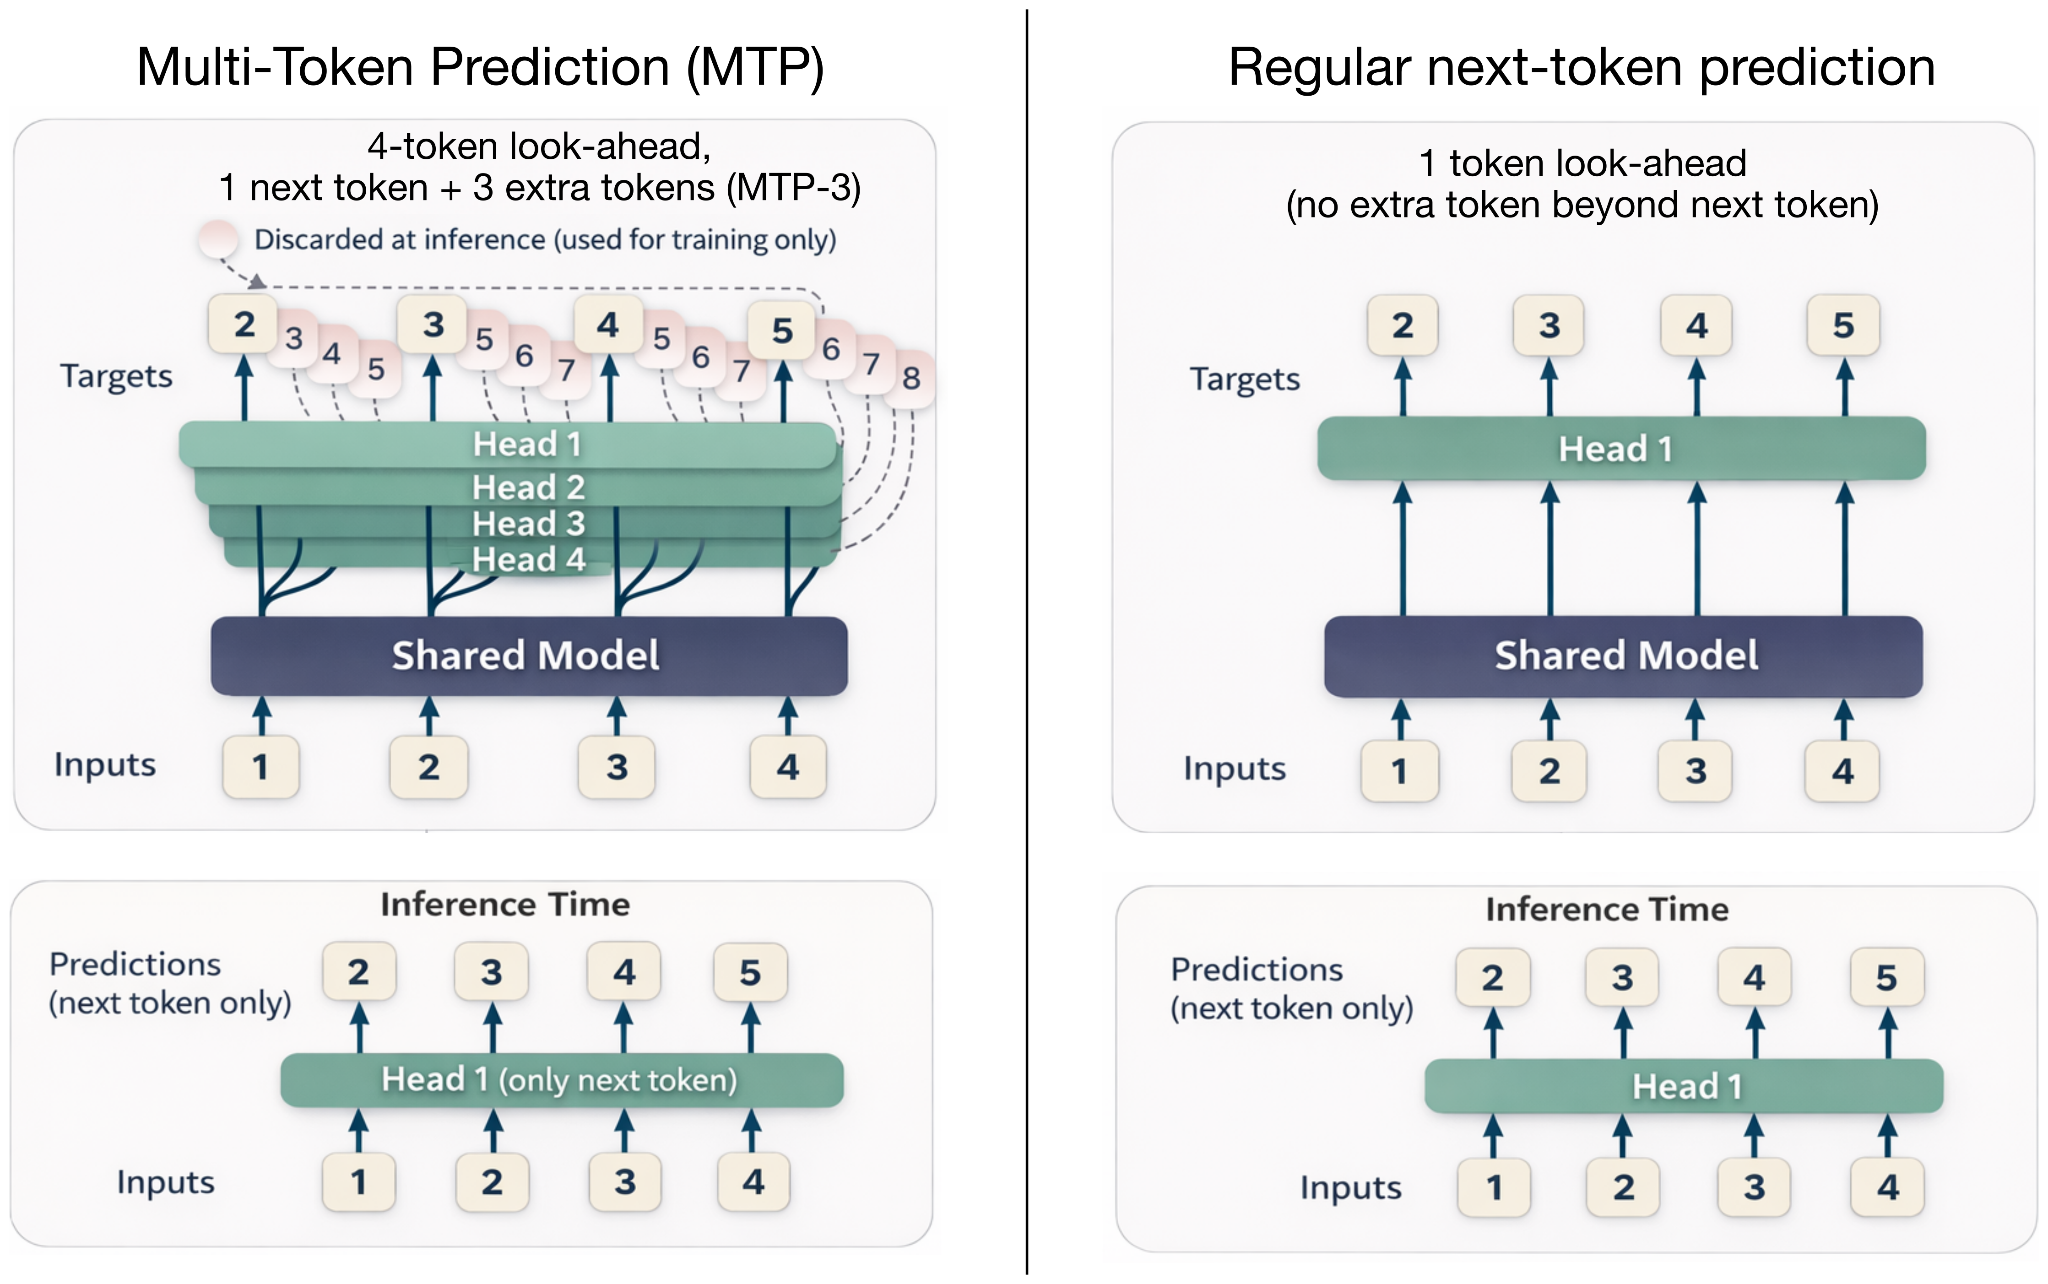
\includegraphics[width=0.6\textwidth]{img/mtp-next-token-vs-multi-token.png}
	\end{center}

	\begin{itemize}
		\item Each head: Linear(hidden\_dim, vocab\_size) --- same as \texttt{lm\_head}
		\item Qwen3-0.6B + 4 heads: 596M + 467M params
		\item In production (DeepSeek-V3): $\sim$1.8$\times$ speedup
	\end{itemize}

\end{frame}

% ────────────────────────────────────────────────────────────────────────────
\begin{frame}{MTP Inference Flow}

	\textbf{One forward pass $\rightarrow$ $n$ tokens!}

	\begin{enumerate}
		\item Run trunk $\rightarrow$ get hidden state $h_t$
		\item Run all $n$ heads in parallel $\rightarrow$ predictions for $t+1, t+2, \ldots, t+n$
		\item Accept tokens greedily (or verify with confidence threshold)
		\item Continue from position $t+n$ (skip $n-1$ decode steps)
	\end{enumerate}

	\begin{block}{Comparison with Speculative Decoding}
		\begin{itemize}
			\item Speculative: needs a separate draft model (extra memory + complexity)
			\item MTP: model is its own draft (only adds small projection heads)
			\item Both reduce the number of autoregressive decode steps
		\end{itemize}
	\end{block}

	\begin{alertblock}{Limitation}
		MTP heads must be trained on multi-token targets.\\
		Randomly initialized heads produce garbage predictions.
	\end{alertblock}

\end{frame}

% ────────────────────────────────────────────────────────────────────────────
\begin{frame}{MTP Training Objective}

	\begin{columns}[T]
		\begin{column}{0.48\textwidth}
			\begin{block}{Standard Training}
				\begin{itemize}
					\item Single prediction head
					\item Target: next token $t+1$
					\item Loss: cross-entropy on $t+1$
				\end{itemize}
				\begin{align*}
					\mathcal{L} &= -\log P(x_{t+1} | x_{\leq t})
				\end{align*}
			\end{block}
		\end{column}
		\begin{column}{0.48\textwidth}
			\begin{block}{MTP Training}
				\begin{itemize}
					\item Multiple prediction heads
					\item Targets: $t+1, t+2, \ldots, t+n$
					\item Combined loss across all heads
				\end{itemize}
				\begin{align*}
					\mathcal{L} &= \sum_{i=1}^{n} w_i \cdot \mathcal{L}_i \\
					\mathcal{L}_i &= -\log P(x_{t+i} | x_{\leq t})
				\end{align*}
			\end{block}
		\end{column}
	\end{columns}

	\begin{block}{Key Difference}
		MTP heads learn to predict \textbf{multiple future tokens} from the same hidden state.\\
		This requires the model to encode richer predictive information.
	\end{block}

\end{frame}

% ────────────────────────────────────────────────────────────────────────────
\begin{frame}{MTP vs Speculative Decoding}

	\begin{center}
		\small
		\begin{tabular}{@{}lcc@{}}
			\toprule
			\textbf{Aspect} & \textbf{MTP} & \textbf{Speculative} \\
			\midrule
			Draft model       & Built-in         & Separate small model    \\
			Training cost     & Higher (multi-head) & Train draft separately \\
			Inference memory  & +small heads     & +full draft model       \\
			Speedup           & $\sim$1.5-2$\times$ & $\sim$2-3$\times$      \\
			Quality           & Same as base     & May differ (draft bias) \\
			Complexity        & Lower            & Higher (verify logic)   \\
			\bottomrule
		\end{tabular}
	\end{center}

	\begin{block}{When to Use Which?}
		\begin{itemize}
			\item \textbf{MTP}: When you can train/finetune the model, memory-constrained
			\item \textbf{Speculative}: When using frozen models, need maximum speedup
		\end{itemize}
	\end{block}

\end{frame}


% ────────────────────────────────────────────────────────────────────────────
\begin{frame}{Real-World Serving Systems}

	\begin{center}
		\small
		\begin{tabular}{@{}lp{5cm}l@{}}
			\toprule
			\textbf{System} & \textbf{Key Features} & \textbf{KV Optimization} \\
			\midrule
			vLLM            & PagedAttention, continuous batching & Block-based KV mgmt \\
			TensorRT-LLM    & Graph optimization, quantization    & FP8 KV, page attention \\
			SGLang          & RadixAttention, structured output   & KV cache reuse \\
			TGI             & Multi-device, streaming             & Efficient batching \\
			\bottomrule
		\end{tabular}
	\end{center}

	\begin{block}{vLLM (Most Popular)}
		\begin{itemize}
			\item PagedAttention eliminates memory fragmentation
			\item Continuous batching: process requests as they arrive
			\item 2-24$\times$ throughput improvement over naive serving
		\end{itemize}
	\end{block}

\end{frame}

% ────────────────────────────────────────────────────────────────────────────
\begin{frame}{Performance Benchmarking}

	\textbf{Key Metrics} for LLM inference:

	\begin{columns}[T]
		\begin{column}{0.48\textwidth}
			\begin{block}{Latency Metrics}
				\begin{itemize}
					\item \textbf{TTFT} (Time to First Token): How long until response starts
					\item \textbf{TPOT} (Time Per Output Token): Average time per token
					\item \textbf{Latency} = TTFT + (tokens $\times$ TPOT)
				\end{itemize}
			\end{block}
		\end{column}
		\begin{column}{0.48\textwidth}
			\begin{block}{Throughput Metrics}
				\begin{itemize}
					\item \textbf{Tokens/sec}: Total tokens generated per second
					\item \textbf{Requests/sec}: Number of completed requests
					\item \textbf{Concurrency}: How many requests handled simultaneously
				\end{itemize}
			\end{block}
		\end{column}
	\end{columns}

	\begin{alertblock}{Trade-off}
		Higher batch size $\rightarrow$ better throughput, but higher latency per request.\\
		Optimal batch size depends on SLA requirements.
	\end{alertblock}

\end{frame}

% ────────────────────────────────────────────────────────────────────────────
\begin{frame}{Summary}

	\begin{enumerate}
		\item \textbf{Two-stage pipeline}: Prefill (compute-bound) vs Decode (memory-bound)
		\item \textbf{Arithmetic intensity}: Decode loads entire model for 1 token $\rightarrow$ very inefficient
		\item \textbf{Decoding strategies}: Temperature, Top-K, Top-P control diversity vs determinism
		\item \textbf{KV-Cache}: Essential optimization --- cache past K/V to avoid $O(s^2)$ recomputation
		\item \textbf{GQA}: Halves KV-Cache size with minimal quality loss
		\item \textbf{Long-context bottleneck}: KV-Cache dominates memory at 32K+ tokens
		\item \textbf{MTP}: Predict multiple tokens per pass --- no separate draft model needed
		\item \textbf{Advanced techniques}: PagedAttention, Flash Attention, quantization enable efficient serving
	\end{enumerate}

	\begin{block}{Experiment Further}
		\begin{itemize}
			\item Train MTP heads and measure real speedup
			\item Try FP8 KV-Cache quantization
			\item Compare streaming latency (TTFT vs TPS)
			\item Benchmark vLLM vs naive serving
		\end{itemize}
	\end{block}

\end{frame}

% ────────────────────────────────────────────────────────────────────────────
\begin{frame}{Further Reading}

	\begin{itemize}
		\item \textbf{FlashAttention}: Fast and Memory-Efficient Exact Attention (Dao et al., 2022)
		\item \textbf{vLLM}: Easy LLM Inference Serving (Kwon et al., 2023)
		\item \textbf{DeepSeek-V3}: Multi-Token Prediction (DeepSeek, 2024)
		\item \textbf{GQA}: Training Generalized Multi-Query Models (Ainslie et al., 2023)
		\item \textbf{PagedAttention}: vLLM's memory management technique
	\end{itemize}

	\begin{block}{Resources}
		\begin{itemize}
			\item GitHub: github.com/vllm-project/vllm
			\item HuggingFace: huggingface.co/docs/transformers
			\item AMD ROCm: rocm.software
		\end{itemize}
	\end{block}

\end{frame}



\end{document}
